%In order to make decisions based on images it is important to recognize objects.
In order to track an marker, it is important to detect these on an image when displayed.
%In order to test out different methods to find features, three different image markers were selected.
% Three image markers are given and the task is to find points that can represent the marker in the image.
In figure \ref{fig:markers} can the different markers to be tracked be seen.
In the simulation, the ideal marker is used but the markers will be tested on a set of real images where lighting, rotation and translation makes the markers harder to detect.
The detector should evaluate the image and return whether the marker was found, and either the center of the marker or several fixed points on the marker.
The detector should be invariant to translation, rotation and projection.
The goal is to use this to track a marker with a robot, keeping the marker in the center of the image and maintain the same distance.
Thus complete invariance to scaling is not a priority, but it should handle small changes in scaling.

\begin{figure}[h]
\centering
 \begin{subfigure}[b]{0.3\linewidth}
 \centering
 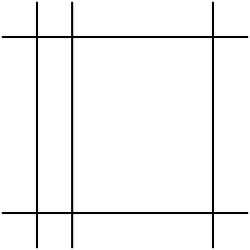
\includegraphics[width=\linewidth]{graphics/Marker2a}
 \caption{Lines}
 \label{marker:cross}
 \end{subfigure}~
 \begin{subfigure}[b]{0.3\linewidth}
 \centering
 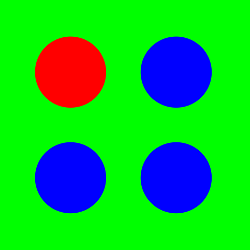
\includegraphics[width=\linewidth]{graphics/Marker1}
 \caption{Circles}
 \label{marker:circle}
 \end{subfigure}
 \begin{subfigure}[b]{0.3\linewidth}
 \centering
 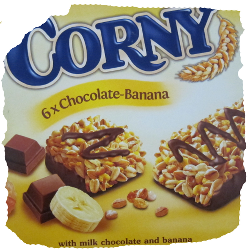
\includegraphics[width=\linewidth]{graphics/Marker3}
 \caption{Corny}
 \label{marker:corny}
 \end{subfigure}
 \caption{The different markers.}
 \label{fig:markers}
\end{figure}

% A full description of the choices and methods used to find the markers can be found in appendix \ref{app:full_vision_part}.